\section{Forschungsmethode}
\label{sec:Forschungsmethode}
Den Richtlinien in \cite{Keele2007GuidelinesEngineering} folgend, wurde ein Systematisches Literatur Review (SLR) nach Kitchenham et al. durchgeführt. Das Dokument folgt dem Aufbau in \cite{Walia2009AErrors} und umfasst die folgenden Schritte 

\begin{itemize}
    \item Formulierung eines Review-Protokolls
    \item Durchführen des Reviews
        \begin{itemize}
            \item Identifizierung von Primärstudien
            \item Evaluierung \& Auswahl
            \item Datenextraktion
            \item Datensynthese
        \end{itemize}
    \item Analyse der Ergebnisse
    \item Auswertung der Ergebnisse
    \item Diskussion der Ergebnisse
\end{itemize}

Ein Review Protokoll enthält alle Forschungsfragen, Methoden, Vorgehensweisen etc. die benötigt werden um ein SLR durchführen zu können Es wird im Vorfeld des Reviews angefertigt, um zu vermeiden, dass das Review durch die Erwartungshaltung des Forschers getrieben wird und damit an Objektivität verliert (Reseracher bias). Nach Durchführung des Reviews wird aus den Ergebnissen der Datensynthese eine Analyse und Auswertung der Ergebnisse durchgeführt um die gestellten Forschungsfragen beantworten zu können \cite{Walia2009AErrors}.

\subsection{Forschungsfragen}

Das zentrale Ziel dieses SLR war es, Qualitätsprobleme im Management der Requirements Traceability und mögliche Lösungsanasätze zu identifizieren und zu klassifizieren. Die zugehörige Fragestellung für den Review war also


\enquote{Welche Arten von Qualitätsprobleme existieren im Management der Requiremenst Traceability und wie können diese behoben werden?}

Zur Beantwortung der Fragestellung, war es notwendig entsprechende Forschungsfragen zu definieren, die sich auf die Beantwortung dieser Fragestellung fokussierten und damit im Review auch zu verwertbaren Ergebnissen führten. Nach einer ersten Analyse des Forschungsgebietes, konnte festgestellt werden, dass ein Teil der Forschungsarbeiten sich nur indirekt auf Qualitätsprobleme im Management von Requirements Traceability bezogen. Im Fall, dass ein Lösungsansatz zur Thematik genannt worden ist, war dieser nicht zwingend nur für den speziellen Anwendungsfall einsetzbar.

Aus den Ergebnissen der Analyse konnte eine Vorgehensweise identifiziert werden, die die Beobachtungen wiederspiegelte und im Einklang mit dem Forschungsfrage dieses Reviews stand. Die Abbildung \ref{fig:abb_forschungsfragen} zeigt das Ergebnis der ersten Analysephase und damit die Festlegung der Vorgehensweise für den weiteren Reviewverlauf

\begin{figure}[!htb]
  \centering
  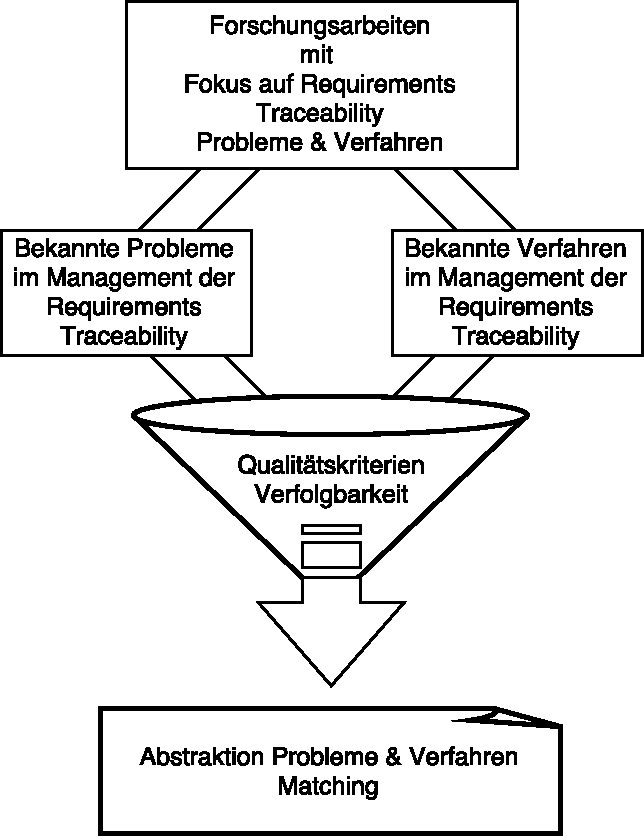
\includegraphics[width=2in]{forschungsfragen_diagramm_v2.pdf}
  \caption{Vorgehensweise zur Beantwortung der Forschungsfragen}
  \label{fig:abb_forschungsfragen}
\end{figure}


% Ggf. anhand des Forschungsziels nochmal zu präzisieren!
Wie in \ref{fig:abb_forschungsfragen} dargestellt wurde das Vorgehen in mehrere Etappen eingeteilt. Im ersten Schritt stand die Identifikation von Forschungsarbeiten die im Themengebiet Requirements Traceability angesiedelt waren und sich mit Problemen oder Lösungsansätzen in diesem Bereich beschäftigten. Entsprechend mussten die Forschungsfragen und Auswahlkriterien so formuliert werden, dass die entsprechenden Arbeiten erfasst wurden. Anhand der Analyse wurde sich dazu entschieden, im weiteren Verlauf Probleme und Verfahren zu separieren und in Bezug zu den Qualitätskriterien zu stellen, da nach der Analyse nicht jeder Lösungsansatz auf einen Anwendungsfall beschränkt ist. Im letzten Schritt folgte dann eine Zusammenführung aller Daten um die Abdeckung von Problemen und Verfahren zu bestimmen um die zentrale Forschungsfrage beantworten zu können.

Die Tabelle \ref{tab:forschungsfragen} zeigt die Forschungsfragen, die aus der Vorgehensweise und der zentralen Fragestellung für diesen Review extrahiert wurden. Um Willkür zu vermeiden, wurde in Tabelle \ref{tab:motivationen} zu jeder Frage eine Motivation niedergeschrieben, die die Sinnhaftigkeit einer Frage separat darstellt. Die erste Frage befasst sich mit möglichen Qualitätsproblemen im Management der Requirements Traceability mit dem Ziel, diese möglichst vollständig zu erfassen. Die zweite Frage befasst sich separat mit den Verfahren zu Behandlung von Qualitätsproblemen und Hinweisen dazu in den erfassten Forschungsarbeiten. Die dritte und letzte Frage fasst die gesammelten Daten zu abstrakteren Vorgehensweisen zusammen, anhand derer ein Abdeckungsgrad für die Problemklasse identifiziert werden kann. Für die Fragen 1-2 war es notwendig einen systematischen Literaturreview durchzuführen. 

\subsection{Suchstring}

Anhand der Analyse war bekannt das Lösungsansätze und Problemen in der Forschungsliteratur korrelieren. Daher reichte ei

Daher wurde ein gemeinsamer Suchstring bestimmt anhand dessen 

Die letzte Frage hat das Ziel, anhand der gesammelten Daten, Verfahren zu identifizieren, anhand dessen ein Abdeckungsgrad bestimmt werden kann.

identifizieren um eine Aussage über die Abdeckbarkeit de

Die erste Frage 


Beschreibung und Grafik über die Forschungsmethode
    Dekomposition in mehrere Forschungsfragen
        Über die Fragen
        
        
    Kombination im Review

Dazu gehörige Forschungsfragen und Motivationen

\begin{table*}[t]
\renewcommand{\arraystretch}{1.3}

\centering
\begin{tabularx}{\textwidth}{@{}X@{}}
\toprule
Forschungsfragen \\ \midrule
1. Welche Arten von Qualitätsproblemen können während des Softwarelebenszyklus im Management der Requirements Traceability entstehen? \\
\hspace*{10mm}1.1 Welche Arten von Qualitätsproblemen in der Requirements Traceability wurden in der vorhandenen Literatur identifiziert? \\
\hspace*{10mm}1.2 Welche Qualitätsprobleme können durch die Analyse ihrer Ursache identifiziert werden? \\
\hspace*{10mm}1.3 Beeinflussen die gefundenen Probleme die Kriterien in \ref{tab:qualitaet_verfolgbarkeit}? \\
2. Welche Verfahren existieren im Management der Requirements Traceability zur Behandlung von Qualitätsproblemen? \\
\hspace*{10mm}2.1 Greift die Literatur Prozesse oder Methodiken auf, die zu einer Verbesserung der Qualität beitragen? \\
\hspace*{10mm}2.2 Addressieren die gefundenen Verfahren die Kriterien in \ref{tab:qualitaet_verfolgbarkeit}? \\
3. Lassen sich die Erkenntnisse aus 1-2 zu Aussagen über mögliche Verfahrensweisen im spezifischen Anwendungsfall zusammenfassen? \\
\bottomrule
\end{tabularx}
\caption{Definierte Forschungsfragen}
\label{tab:forschungsfragen}
\end{table*}

\begin{table*}[t]
    \centering
    \begin{tabularx}{\textwidth}{X}
        \toprule
        Motivationen \\ \midrule
        1. Unabhängige Erfassung aller Qualitätsprobleme die mindestens eine der Kriterien für Qualität von Verfolgbarkeit beinflussen \\
        2. Unabhängige Erfassung aller Verfahren die mindestens einer der Kriterien für Qualität von Verfolgbarkeit beeinflussen \\
        3. Bestimmen von Verfahren und ihrer Abdeckung für die Behandlung von Qualitätsproblemen \\
    \bottomrule
    \end{tabularx}
    \caption{Motivationen zu den gestellten Forschungsfragen in \ref{tab:forschungsfragen}}
    \label{tab:motivationen}
\end{table*}

\subsection{Auswahl von Quellen und Suchkriterien}

Über die Auswahl der Datenquellen
    Kriterien
    
Liste von Datenquellen

\begin{table}[!ht]
\renewcommand{\arraystretch}{1.3}
\centering
\begin{threeparttable}
\begin{tabularx}{\columnwidth}{@{}lX@{}}
\toprule
Kriterium & Auswirkung\\ \midrule
Datenbanken & ACM Digital Library, IEEE Xplore, Science Direct (Elsevier), SpringerLink\\
Andere Artikel & SWEBOK - Software Engineering Body of Knowlege\\
Erweiterte Quellen & Buchquellen \\
\bottomrule
\end{tabularx}
\medskip
      %\footnotesize\textbf{Legende:}\smallskip
      %\begin{tablenotes}\footnotesize
      %\item[*] In \cite{Kollanus2010Test-DrivenApproach} werden die gleichen Studien wie in \cite{Kollanus2011CriticalDevelopment} untersucht.
      %\end{tablenotes}
\end{threeparttable}
\caption{Quellen für den Review}
\label{tab:quellen_review}
\end{table}

    
Review zur Vermeidung von BIAS

Wie wurden die gefundenen Quellen ausgewählt
    Vorgehen Titel, Abstract, Inklusion...
    
Liste Inklusions- und Exklusionkriterien

\begin{table}[!ht]
\renewcommand{\arraystretch}{1.3}
\centering
\begin{threeparttable}
\begin{tabularx}{\columnwidth}{@{}XX@{}}
\toprule
Inklusionskriterien & Exklusionskriterien \\ \midrule
Studie beschäftigt sich mit Problemen in der Requirements Traceability & Studie hat keinen Bezug zum Forschungsgebiet \\
Studie beschäftigt sich mit Ursachen für Problemen in der Requirements Traceability & Studie hat keinen Bezug zu den gestellten Forschungsfragen \\
& Studie ist nicht auf Englisch \\
& Ergebnisse einer Studie sind unklar oder mehrdeutig \\
\bottomrule
\end{tabularx}
\medskip
      %\footnotesize\textbf{Legende:}\smallskip
      %\begin{tablenotes}\footnotesize
      %\item[*] In \cite{Kollanus2010Test-DrivenApproach} werden die gleichen Studien wie in \cite{Kollanus2011CriticalDevelopment} untersucht.
      %\end{tablenotes}
\end{threeparttable}
\caption{Inklusions- und Exklusionkriterien}
\label{tab:inklusions_exklusionkriterien}
\end{table}

Liste Qualitätskriterien

\begin{table}[!ht]
\renewcommand{\arraystretch}{1.3}
\centering
\begin{threeparttable}
\begin{tabularx}{\columnwidth}{@{}XX@{}}
\toprule
Qualitätskriterien \\ \midrule
Ist die Studie in sich schlüssig? \\
Basiert die Studie auf sinnvollen Annahmen? \\
Ist die Vorgehensweise angemessen? \\
Werden in der Studie Maßnahmen angewendet, um Mehrdeutigkeiten zu vermeiden? \\
Kann die Studie nachvollzogen werden? \\
\bottomrule
\end{tabularx}
\medskip
      %\footnotesize\textbf{Legende:}\smallskip
      %\begin{tablenotes}\footnotesize
      %\item[*] In \cite{Kollanus2010Test-DrivenApproach} werden die gleichen Studien wie in \cite{Kollanus2011CriticalDevelopment} untersucht.
      %\end{tablenotes}
\end{threeparttable}
\caption{Qualitätskriterien}
\label{tab:qualitaetskriterien}
\end{table}

Über die Auswahl der Papiere, Wieviele gefunden, Auswahl nach Titel etc.
Über die Qualität der Papiere

Liste Verteilung de Papiere?

\subsection{Datenextraktion und Datensynthese}

Extrahiere Items, passend zu Fokus



BIAS vermeidung?

\subsection{Reporting des Reviews}

Beantworten der einzelnen Forschungsfragen

\section{Diskussion}

Grafik zu

Das Hauptaugenmerk dieses SLR war es, bestehende Probleme in der Requirements Traceability zu identifizieren und zu klassifizieren. Um einen Fokus zu setzen, wurde sich bei den Forschungfragen am untergeordneten Ziel, der Verbesserung der Erkennung und Vermeidung von Qualitätsproblemen in der Requirements Traceability, orientiert. Unter betrachtung 

Das Hauptziel dieses Reviews war:

\begin{center}
\enquote{Welche Arten von Problemen entstehen im Management der Requirements Traceability und wie können diese klassifiziert werden?}
\end{center}

-------------



\subsection{Ablauf (Review, Suchprozess)}

Review planen:

Forschungsfragen
Review Protokoll

Review ausführen:

Suchstrategie, Suchprozess, Methodik
Dokumentierung der Suche

Review Protokoll

Bestehende SLRs
Generellese Forschungsfeld
Zitationen von Gotel \& Finkelstein

\subsection{Kriterien (Inkusion-, Exklusion)}

Was sind die Kriterien für die Inkusion- / Exklusion- von Disserationen

\subsection{Analyse}

Wie wird analysiert, was sind die Methoden?
